\section{Implementation}
\label{sec:implementation}

% \begin{itemize}
%   \item Extension of the library RxLua
%   \item Why reactive?
%     \url{http://www.reactivemanifesto.org/}
%   \item ØMQ Lua bindings
%   \item ØMQ queues with push/pull protocol - Fire-and-forget messaging: a messsaging pattern in which we do not expect a direct response to the message, as opposed to request-response protocols
% \end{itemize}

Stream processings are more and more designed as reactive.

On September 2014 has been published the Reactive Manifesto\cite{reactivemanifesto}.
This one attempts to define the principles to build systems more flexible, loosely-coupled and scalable.
A reactive system has to follow the four Reactive Principles:

\begin{itemize}
  \item Responsive: it is quick to react to all users in order to ensure a consistently positive user experience;
  \item Elastic: it is easily upgraded on demand in order to ensure responsiveness under various load conditions;
  \item Resilient: it applies proper design and architecture principles in order to ensure responsiveness;
  \item Message-driven: it is based on a message-passing architecture to establish a boundary between components that ensures loose coupling, isolation and location transparency, e.g. event-driven, actor-based, or both of them.
\end{itemize}

The responsiveness of a system needs both elasticity and resiliency.
Finally, a message-driven architecture is the foundation of elastic, resilient and responsive systems\ref{fig:reactive-traits}.

\begin{figure}[t!]
  \centering
  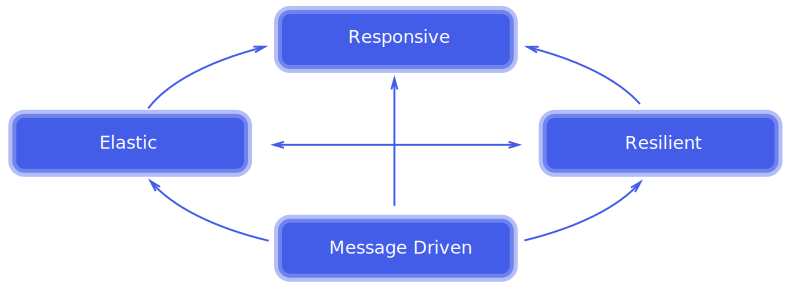
\includegraphics[width=.99\linewidth]{images/reactive-traits}
  \caption{Reactive traits.}
  \label{fig:reactive-traits}
\end{figure}




\begin{minipage}{\linewidth}
\begin{lstlisting}[language=LUA,caption={Process pipeline example, using the library RxLua},label=pipeline-example]
Rx.Observable.fromTable(people)
 :map(
   function(person)
     return person.age
   end
 )
 :filter(
   function(age)
     return age > 18
   end
 )
 :reduce(
   function(accumulator, age)
     accumulator[count] = (accumulator.count
       or 0) + 1
     accumulator[sum] = (accumulator.sum
       or 0) + age
     return accumulator
   end, {}
 )
 :subscribe(
   function(datas)
     print("Adult people average:",
       datas.sum / datas.count)
   end,
   function(err)
     print(err)
   end,
   function()
     print("Process complete!")
   end
 )
\end{lstlisting}
\end{minipage}
